\documentclass{standalone}
\usepackage{../../../../preamble_formulas}

\begin{document}
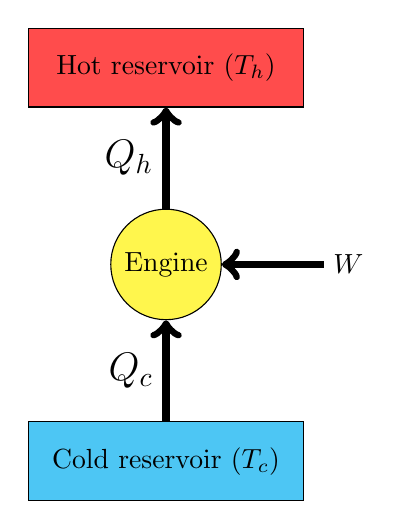
\begin{tikzpicture}
  \node[rectangle,
    draw = black,
    fill = red!70,
    minimum width = 3.5cm,
    minimum height = 1cm] (hot) at (0,2.5) {Hot reservoir ($T_\text{h}$)};
  \node[rectangle,
    draw = black,
    fill = cyan!70,
    minimum width = 3.5 cm,
    minimum height = 1cm] (cold) at (0,-2.5) {Cold reservoir ($T_\text{c}$)};
  \node[circle,draw,fill=yellow!70,minimum size = 1cm] (engine) at (0,0){Engine}; %minimum size = diameter of the circle.

  \node[anchor=west] (w) at (2,0) {$W$};

  %\nucleus{gray}{Tl}{6}{-18}{208}{81}{3.1}{minutes}
  \draw[<-,font=\Large,line width=1mm] (hot.south) -- node[left]{$Q_\text{h}$} (engine.north);
  \draw[<-,font=\Large,line width=1mm] (engine.south) -- node[left]{$Q_\text{c}$} (cold.north);
  \draw[<-,font=\Large,line width=1mm] (engine.east) -- (w.west);

\end{tikzpicture}
\end{document}